\section[Фигура 1]{Фигура 1}
Используя примитивы \textbf{Inkscape}, строим окружности. 
Применяем операцию \textit{\textbf{Union (объединение)}} для получения требуемой фигуры.

\hspace{0pt}
\begin{figure}[H]
    \begin{minipage}[h]{0.47\linewidth}
        \center{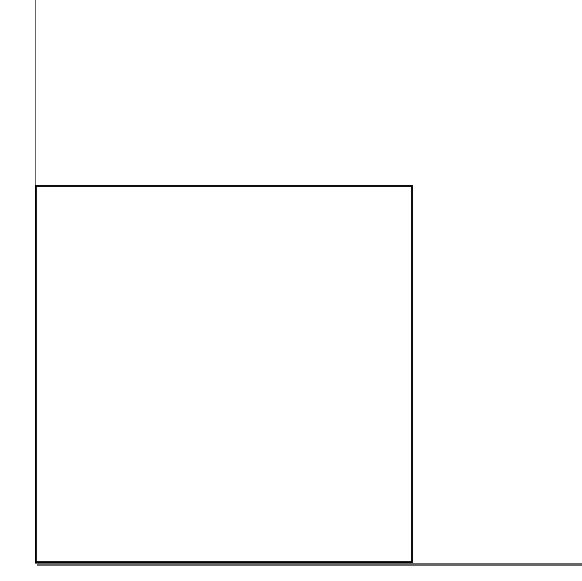
\includegraphics[width=1\linewidth]{1_1_create.png}} Создание фигур\\
    \end{minipage}
    \hfill
    \begin{minipage}[h]{0.47\linewidth}
        \center{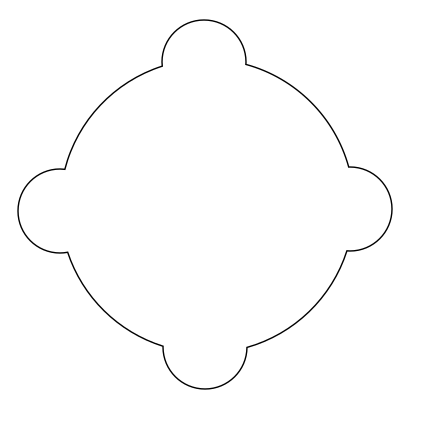
\includegraphics[width=1\linewidth]{1_2_union.png}} \\Операция Union
    \end{minipage}
    \hfill
\end{figure}
